	\documentclass[10pt,oneside]{CBFT_book}
	% Algunos paquetes
	\usepackage{amssymb}
	\usepackage{amsmath}
	\usepackage{graphicx}
	\usepackage{libertine}
	\usepackage[bold-style=TeX]{unicode-math}
	\usepackage{lipsum}

	\usepackage{natbib}
	\setcitestyle{square}

	\usepackage{polyglossia}
	\setdefaultlanguage{spanish}


	\usepackage{CBFT.estilo} % Cargo la hoja de estilo

	% Tipografías
	% \setromanfont[Mapping=tex-text]{Linux Libertine O}
	% \setsansfont[Mapping=tex-text]{DejaVu Sans}
	% \setmonofont[Mapping=tex-text]{DejaVu Sans Mono}

	%===================================================================
	%	DOCUMENTO PROPIAMENTE DICHO
	%===================================================================

\begin{document}

% =================================================================================================
\chapter{Fenómenos dependientes del tiempo}
% =================================================================================================

% =================================================================================================
\section{Ley de Faraday e inducción}
% =================================================================================================

\[
	\mathcal{E} = -\frac{1}{c} \frac{d}{dt}\left( \int_S \vb{B}\cdot d\vb{S} \right)
\]
siendo $S=\partial\Gamma$ y donde 
\[
	\mathcal{E} \equiv \int_\Gamma \vb{E}\cdot d\vb{\ell}
\]
siendo \vb{E} un campo irrotacional medido en el frame donde $\Gamma$ está en reposo.
El signo menos es la ley de lenz, la FEM se opone el cambio de flujo.

Pero la variación de flujo puede deberse a variación de \vb{B} o a deformación del circuito.
\[
	\frac{d}{dt}\int_S \vb{B}\cdot d\vb{S} = \int_S \dpar{\vb{B}}{t}\cdot d\vb{S} +
	\int_\Gamma \vb{B}\times\vb{V} \cdot d\vb{\ell}
\]
y entonces
\[
	\int_\Gamma \vb{E}'\cdot d\vb{\ell} = -\frac{1}{c} \int_S \dpar{\vb{B}}{t}\cdot d\vb{S} +
	\frac{1}{c} \int_\Gamma \vb{B}\times\vb{V} \cdot d\vb{\ell}
\]
\[
	\int_\Gamma [\vb{E}'- \vb{B}\times\vb{V} ] \cdot d\vb{\ell} = -\frac{1}{c} \int_S \dpar{\vb{B}}{t}\cdot d\vb{S}
\]
y si $\vb{E} = \vb{E}'- \vb{B}\times\vb{V}$ es el campo medido en el laboratorio se llega a la 
ley de Faraday,
\[
	\int_\Gamma \vb{E}\cdot d\vb{\ell} = -\frac{1}{c} \int_S \dpar{\vb{B}}{t}\cdot d\vb{S}
\]
y usando el teorema de Stokes a su forma diferencial
\[
	\rotorm{E} = -\frac{1}{c} \dpar{\vb{B}}{t}
\]
siendo este campo \vb{E} claramente no conservativo.

\subsection{Corrección a las ecuaciones}

Entonces resultan las siguientes cuatro ecuaciones
\[
	\divem{D} = 4 \pi \rho \qquad \qquad \rotorm{E} = \frac{1}{c} \dpar{\vb{B}}{t}
\]
que son las leyes de Coulomb y Faraday en forma diferencial. Asimismo
\[
	\divem{B} = 0 \qquad \qquad \rotorm{H} = \frac{4\pi}{c} \vb{J}
\]
que es la no existencia de monopolos magnéticos y la ley de Ampere. En el último caso con $\divem{J}=0$
que es para corrientes estacionarias.

Justamente por ello la ecuación relacionada con la ley de Ampere está incompleta así puesto que se dedujo
para corrientes estacionarias. Maxwell introduce la continuidad aproximadamente en 1865.
Entonces, como 
\[
	\divem{J} + \dpar{\rho}{t } = 0 
\]
se sigue que 
\[
	\divem{J} + \frac{\partial}{\partial t} \frac{\divem{D}}{4\pi} =
	\Nabla\cdot\left[ \vb{J} + \frac{1}{4\pi} \dpar{D}{t} \right]
\]
que es posible pensar como una nueva densidad de corriente \vb{J}. 
Entonces la ley de Ampere completa es:
\[
	\rotorm{H} = \frac{4\pi}{c} \vb{J} + \frac{1}{c}\dpar{D}{t}
\]
siendo $\dpar{D}{t}$ la llamada corriente de desplazamiento. 
Las cuatro ecuaciones están ahora completas y constituyen las {\it ecuaciones de Maxwell}.

\subsection{Potenciales}

\be
	\divem{D} = 4 \pi \rho \qquad \qquad \rotorm{E} = \frac{1}{c} \dpar{\vb{B}}{t}
	\label{maxwell_e}
\ee
\be
	\divem{B} = 0 \qquad \qquad \rotorm{H} = \frac{4\pi}{c} \vb{J} + \frac{1}{c}\dpar{D}{t}
	\label{maxwell_m}
\ee
Dado que $\divem{B} = 0$ al igual que en magnetostática, podemos derivar \vb{B} del potencial 
vector \vb{A}, pero \vb{E} no tiene rotor nulo, entonces no existe $\phi$ potencial escalar.

Tomando
\[
	\rotorm{E} + \frac{1}{c}\dpar{D}{t} = \rotorm{E} + \frac{\partial}{\partial t}\left( \frac{1}{c} 
	\rotorm{A}\right) = \Nabla\times\left[ \vb{E} + \frac{1}{c}\dpar{\vb{A}}{t}\right] = 0
\]
podemos pensar en un potencial general $\Phi$ tal que 
\[
	- \Nabla \Phi = \vb{E} + \frac{1}{c}\dpar{\vb{A}}{t}
\]
o bien 
\[
	\vb{E}  = -\Nabla \Phi - \frac{1}{c}\dpar{\vb{A}}{t},
\]
donde por supuesto $\Phi$ no tiene significado de trabajo como sí lo tenía el potencial
electrostático.

Podemos expresar las ecuaciones \eqref{maxwell_e} y \eqref{maxwell_m} con $\vb{A},\Phi$,
\[
	\divem{E} = 4\pi\rho \rightarrow 
	Nabla\cdot\left( -\Nabla \Phi - \frac{1}{c}\dpar{\vb{A}}{t} \right) = 4\pi\rho
\]
\[
	\rotorm{B} - \frac{1}{c}\dpar{E}{t} =  \frac{4\pi}{c} \vb{J}  \rightarrow
	\Nabla\times(\rotorm{A}) - \frac{1}{c}\frac{\partial}{\partial t}\left( 
	-\Nabla \Phi - \frac{1}{c}\dpar{\vb{A}}{t} \right)=  \frac{4\pi}{c}\vb{J}
\]
de manera que resultan dos ecuaciones para los potenciales, pero acopladas
\[
	\nabla^2 \Phi + \frac{1}{c} \frac{\partial}{\partial t}\divem{A} = -4 \pi \rho
\]
\[
	\nabla^2 \vb{A} - \frac{1}{c^2} \dpar[2]{\vb{A}}{t} -\Nabla \left( \divem{A} + \frac{1}{c}
	\dpar{\Phi}{t} \right) = -\frac{4\pi}{c} \vb{J}
\]

\subsection{Cambio de Gauge}

Podemos desacoplarlas utilizando la arbitrariedad de los potenciales
\be
	\rotorm{A} = \vb{B} \qquad -\Nabla\Phi - \frac{1}{c} \dpar{\vb{A}}{t} = \vb{E}
	\label{ecs_potencial_em}
\ee
si le sumamos una función al potencial vector,
\[
	\vb{A} \rightarrow \vb{A}'= \vb{A} + \Nabla \Lambda,
\]
se da que 
\[
	\rotorm{A} = \rotorm{A'}
\]
pero
\[
	- \Nabla\Phi - \frac{1}{c}\dpar{\vb{A}}{t} - \frac{1}{c}\dpar{\Nabla\Lambda}{t} = \vb{E}
\]
lo cual vale si y sólo si
\[
	-\Nabla\left( \Phi + \frac{1}{c} \dpar{\Lambda}{t} \right) -\frac{1}{c}\dpar{\vb{A}}{t}   = \vb{E}
\]
de manera que requiero 
\[
	\Phi \rightarrow \Phi'= \Phi - \frac{1}{c} \dpar{\Lambda}{t}
\]
y estas dos ecuaciones fijan la transformación de gauge. Como con $\vb{A'}, \Phi'$ siguen valiendo las 
\eqref{ecs_potencial_em}, requiero que 
\[
	\divem{A'} + \frac{1}{c}\dpar{\Phi'}{t} = 0 = \divem{A} + \frac{1}{c}\dpar{\Phi}{t} + \nabla^2 \Lambda
	- \frac{1}{c^2} \dpar[2]{\Lambda}{t}
\]
entonces
\[
	\divem{A} + \frac{1}{c}\dpar{\Phi}{t} = -\left(\nabla^2 \Lambda - \frac{1}{c^2} \dpar[2]{\Lambda}{t}\right)
\]
y si usamos los nuevos potenciales, ahora sin apóstrofes para no confundir con notación redundante,
\[
	\nabla^2 \vb{A} - \frac{1}{c^2}\dpar[2]{\vb{A}}{t} = -\frac{4\pi}{c}\vb{J}
\]
\[
	\nabla^2 \Phi - \frac{1}{c^2}\dpar[2]{\Phi}{t} = -\frac{4\pi}{c}\rho
\]
ambos potenciales satisfacen sendas ecuaciones de onda. El {\it gauge de Lorentz} o ``condición de
Lorentz'' es
\[
	\divem{A} + \frac{1}{c} \dpar{\Phi}{t} = 0.
\]

Podemos imponer también 
\[
	\divem{A} = 0
\]
el gauge de Coulomb y entonces
\[
	\nabla^2 \Phi = -4\pi\rho
\]
vemos que el potencial $\phi$ cumple la ecuación de Poisson.
El campo se describirá como el estacionario (electrostático) entonces
\[
	\dpar{\Phi}{t} = 0
\]
y entonces
\[
	\divem{A} + \frac{1}{c} \dpar{\Phi}{t} = 0
\]
siendo cada uno de los términos nulos por sí mismo.
Los resultados físicos deben ser independientes del gauge.

% =================================================================================================
\section{Conservación de la energía (teorema de Poynting)}
% =================================================================================================

Sea una región con volumen fijo. Existen \vb{E}, \vb{B} solamente que varían con el tiempo.
Pareciera que la energía debiera conservarse.
\[
	\vb{F} = q \left( \vb{E} + \frac{1}{c} \pv{v}{B} \right)
\]
entonces
\[
	\delta W = \vb{F}\cdot d\vb{\ell} = q \vb{E}\cdot d\vb{\ell} 
\]
dado que \vb{B} no hace trabajo por ser perpendicular la fuerza la velocidad.
\[
	\delta U = q \vb{E}\cdot d\vb{\ell} 
\]
para una carga $q$ es
\[
	\dtot{U}{t} = q \vb{E}\cdot \vb{v} 
\]
y para una distribución de cargas,
\[
	\dtot{U}{t} = \int_V \rho \vb{E}\cdot \vb{v}  dV = \int_V \vb{J}\cdot \vb{E} dV
\]
que no es otra cosa que la potencia entregada por los campos \vb{E}, \vb{B} dentro del volumen
$V$. Es una conversión de energía electromagnética en energía mecánica o térmica.

\[
	\int_V \vb{J}\cdot \vb{E} dV = \int_V \left[ \frac{c}{4\pi}(\rotorm{H})\cdot\vb{E} - 
		\frac{1}{4\pi}\dpar{\vb{D}}{t}\cdot\vb{E} \right] dV
\]
Si usamos la identidad
\[
	\Nabla\cdot(\pv{E}{H}) = \vb{H}\cdot(\rotorm{E}) - \vb{E}\cdot(\rotorm{H}),
\]
podemos escribir
\[
	= \int_V \frac{c}{4\pi} \left( \left[ \vb{H}\cdot(\rotorm{E}) - \Nabla\cdot(\pv{E}{H}) \right] - 
		\frac{1}{4\pi}\dpar{\vb{D}}{t}\cdot\vb{E}  \right) dV
\]
\[
	= - \frac{1}{4\pi}\int_V \left[ \vb{H}\cdot\dpar{\vb{B}}{t} + \dpar{\vb{D}}{t}\cdot\vb{E} \right] dV - 
		\int_V \frac{c}{4\pi}  \Nabla\cdot(\pv{E}{H}) dV
\]
\[
	= - \frac{1}{8\pi}\frac{d}{dt} \int_V \left[ \vb{H}\cdot\vb{B} + \vb{D}\cdot\vb{E} \right] dV - 
		 \frac{c}{4\pi} \int_S (\pv{E}{H}) dS
\]
siendo $S\equiv\partial V$. Si denominamos ahora
\[
	\vb{S} \equiv \frac{c}{4\pi}(\pv{E}{H}) \qquad \text{vector de Poynting}
\]
\[
	U = \frac{1}{8\pi}\left( \vb{H}\cdot\vb{B} + \vb{D}\cdot\vb{E} \right) \qquad \text{Densidad de energía EM}
\]
resulta que 
\[
	\pe{J}{E} = -\dpar{U}{t} - \divem{S}
\]
entonces la conservación de la energía por unidad de volumen es
\[
	-\pe{J}{E} = \dpar{U}{t} + \divem{S}
\]
e integrada
\[
	\int_V \dpar{U}{t} dV + \int_V \divem{S} dV = - \int_V \pe{J}{E} dV = -\int_S \vb{S}\cdot d\vb{S}
\]
donde se ha aplicado el teorema de Gauss en el miembro derecho. Así
\[
	\int_V \dpar{U}{t} dV + \int_V \divem{S} dV = -\int_S \vb{S}\cdot d\vb{S}
\]
siendo el primer término del LHS la variación de la energía total, el segundo la potencia entregada por
los campos sobre las fuentes y el RHS el flujo de energía a través de la región transportado por el
vector de Poynting.
Notemos que $\pe{J}{E}$ es el trabajo hecho por unidad de tiempo y por volumen por los campos.
Localmente la conservación de la energía es
\[
	\dtot{U_cam}{t} + \dtot{Umec}{t} = -\int_S \vb{S}\cdot d\vb{S}.
\]
\vb{S} y $U$ no están relacionados linealmente con \vb{E} y \vb{H}.

\subsection{Conservación del momento}

En el discreto se tiene
\[
	\vb{F} = \dtot{\vb{P}}{t} = q\vb{E} + q\frac{1}{c} \pv{v}{B} 
\]
y pasando al continuo
\[
	\dtot{\vb{P}_M}{t} = \int_V \left[ \rho\vb{E} + \frac{1}{c} \pv{J}{B}  \right] dv
\]
\[
	\dtot{\vb{P}_M}{t} = \int_V \left[ \frac{1}{4\pi} (\divem{D}) \vb{E} + 
	\frac{1}{c} \left( \frac{c}{4\pi}\rotorm{H} - \frac{1}{4\pi}\dtot{\vb{D}}{t} \right)\times {B} \right] dv
\]
\[
	\dtot{\vb{P}_M}{t} = \int_V \left[ \frac{1}{4\pi} (\divem{D}) \vb{E} +  
	\frac{1}{4\pi} (\Nabla\times\vb{H}\times\vb{B}) - \frac{1}{4\pi c}\dtot{\vb{D}}{t}\times {B} \right] dv
\]
Ahora, usando las siguientes cuentas auxiliares
\[
	\dpar{}{t}(\pv{D}{B}) = \dpar{\vb{D}}{t}\pv{}{B} + \pv{D}{}\dpar{\vb{B}}{t}
\]
\[
	\epsilon\mu\dpar{}{t}(\pv{E}{H}) = \epsilon\mu\dpar{\vb{D}}{t}\pv{}{B} + \epsilon\mu\pv{D}{}\dpar{\vb{B}}{t}
\]
y ahora volviendo
\[
	\dtot{\vb{P}_M}{t} = \frac{1}{4\pi} \int_V \left[  (\divem{D}) \vb{E} + (\Nabla\times\vb{H}\times\vb{B}) 
	-\frac{1}{c}\epsilon\mu \left( \dpar{}{t}(\pv{E}{H}) - \pv{E}{}\dpar{\vb{H}}{t} \right) \right] dv	
\]
haciendo un pase de miembros y expresando \vb{H} en términos de \vb{E} es
\begin{multline*}
	\dtot{\vb{P}_M}{t} + \frac{\epsilon\mu }{4\pi c} \int_V \dpar{}{t}(\pv{E}{H}) dV = \\
	\frac{1}{4\pi} \int_V \left[  (\divem{D}) \vb{E} - \epsilon \pv{E}{}(\Nabla\times\vb{E}) +
	\rotorm{H}\times\vb{B} + \vb{H}(\divem{B}) \right] dV	 
\end{multline*}
donde el último término en el integrando del RHS es cero y se lo puedo sumar por ello.
Prosiguiendo
\begin{multline*}
	\dtot{\vb{P}_M}{t} + \frac{\epsilon\mu }{4\pi c} \dtot{}{t}\int_V (\pv{E}{H}) dV = \\
	\frac{1}{4\pi} \int_V \left[  (\divem{D}) \vb{E} - \pv{D}{}(\Nabla\times\vb{E}) +
	\vb{H}(\divem{B}) - \vb{B}(\rotorm{H}) \right] dV	
\end{multline*}
y con algunads identidades más
\[
	= \frac{1}{4\pi} \int_V \Nabla\left( \left[ \vb{D}\vb{E} - \frac{1}{2}\mathbb{1}( \pe{D}{E}) \right] + 
		\left[ \vb{H}\vb{B} - \frac{1}{2}\mathbb{1}(\pe{H}{B}) \right] \right) dV
\]
donde los primeros términos dentro de cada corchete son productos tensoriales (su resultado no es un
número sino un tensor).

Hemos encontrado que se puede definir la conservación como flujo de un tensor de segundo rango,
\[
	T_{ik} = \frac{1}{4\pi}\left[ \epsilon E_iE_k + \mu H_iH_k - \frac{1}{2}\delta_{ik}
	( \epsilon E^2 + \mu H^2)\right]
\]
que es el tensor de esfuerzos de Maxwell.

Entonces
\[
	\int_V (\rho\vb{E} + \frac{1}{c}(\pv{J}{B}) ) dV + 
	\dtot{}{t}\left( \frac{1}{4\pi c}\int_V (\pv{D}{B})dV\right) = \int_S T \cdot d\vb{S}
\]
con la normal saliente. Luego, localmente la conservación del momento lineal es
\[
	\dtot{\vb{P}_mec}{t} + \dtot{\vb{P}_cam}{t}  = \int_S T \cdot d\vb{S}
\]
donde el RHS es la fuerza por unidad de área a través de $S$ que actúa sobre las partículas y
los campos dentro de $V$.
Definiendo
\[
	\frac{1}{c^2} \vb{S}=  \vb{g} = \frac{1}{4\pi c}(\pv{D}{B})
\]
se tiene que \vb{g} es una densidad de flujo de momento y también puede expresarse
\[
	\vb{g} = \frac{\epsilon\mu}{4\pi c}(\pv{E}{H}).
\]

Observemos que el tensor de Maxwell es un tensor cartesiano.



% =================================================================================================
\section{Tensor de Maxwell}
% =================================================================================================

El tensor T será diagonal si una de las direcciones es paralela al campo. Con el T puede calcularse
la fuerza que hacen los campos \vb{E}, \vb{B} sobre una cierta distribución de cargas y corrientes,
con tal de evaluar su flujo en alguna superficie que las contenga (como se ve en la figura)
\begin{figure}[htb]
	\begin{center}
	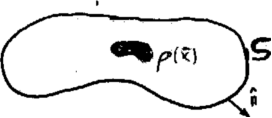
\includegraphics[width=0.4\textwidth]{images/fig_ft1_maxwell.pdf}	 
	\end{center}
	\caption{}
\end{figure} 
y con tal dde que 
\[
	\dtot{}{t}\left(\int_V \vb{g} dV \right) = 0 \qquad \qquad \vb{g} =  \frac{1}{4\pi c}(\pv{E}{B})
\]
puesto que en ese caso será
\[
	\vb{F} = \int_S T \cdot d\vb{S}.
\]

En este caso se suele definir el concepto de presión de radiación
\[
	\vb{R}_rad \equiv \dtot{\vb{F}}{S} T\cdot\hat{n}.
\]

T es un tensor con autovalores reales; coincidiendo sus autovectores con la dirección del campo.
Es independiente del sentido del campo, depende del valor absoluto de los mismos.
\[
	T_{ik} = \frac{1}{4\pi} \left[ \epsilon E_iE_k - \frac{1}{2}\delta_{ik} \epsilon E^2 \right] 
\]
es el tensor eléctrico y
\[
	T_{ik} = \frac{1}{4\pi} \left[ \mu H_iH_k - \frac{1}{2}\delta_{ik} \mu H^2  \right] 
\]
el tensor magnético.

\subsection{Ejemplos del tensor de Maxwell}

Respecto de la figura, donde vemos que el campo penetra en el recinto y la tensión es hacia adentro,
\begin{figure}[htb]
	\begin{center}
	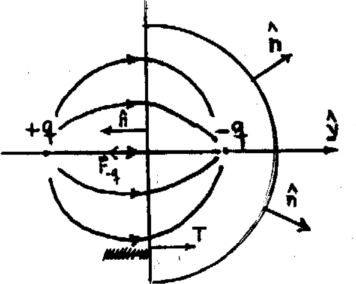
\includegraphics[width=0.4\textwidth]{images/fig_ft1_tensorM1.pdf}
	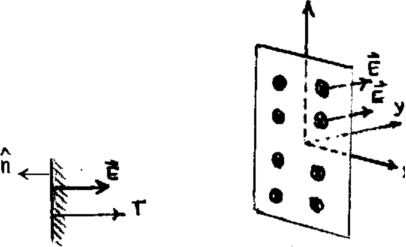
\includegraphics[width=0.5\textwidth]{images/fig_ft1_tensorM2.pdf}	
	\end{center}
	\caption{}
\end{figure} 
escribimos 
\[
	d\vb{S} = -dS\hat{y} \qquad \vb{F}_{\text{sobre}\:-q} = -F\hat{y}
\]
\[
	T|_S = \begin{pmatrix}
	        -E_y^2	& 0 	& 0 \\
		0	& E_y^2	& 0 \\
		0	& 0	& -E_y^2
	       \end{pmatrix}
\]
la fuerza atractiva hacia afuera del recinto.
\begin{figure}[htb]
	\begin{center}
	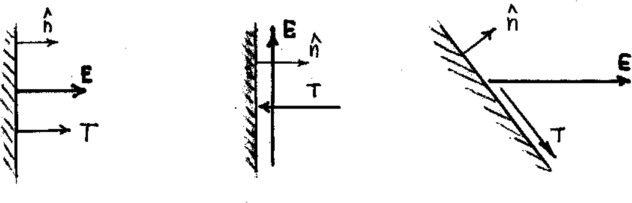
\includegraphics[width=0.8\textwidth]{images/fig_ft1_tensorM3.pdf}	 
	\end{center}
	\caption{}
\end{figure} 

En este otro caso, el campo sale del recinto y la tensión es hacia afuera pués la $\hat{n}$
ha cambiado de sentido.
\[
	T\cdot d\vb{S} \propto \hat{y} \qquad \vb{F}_{\text{sobre}\:+q} = F\hat{y}
\]
es una fuerza atractiva hacia afuera del recinto.
\begin{figure}[htb]
	\begin{center}
	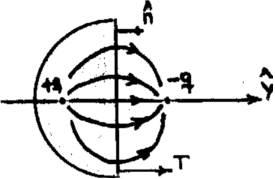
\includegraphics[width=0.4\textwidth]{images/fig_ft1_tensorM4.pdf}	 
	\end{center}
	\caption{}
\end{figure} 

Aquí abajo el campo es tangencial al recinto, la tensión penetra en él.

\begin{figure}[htb]
	\begin{center}
	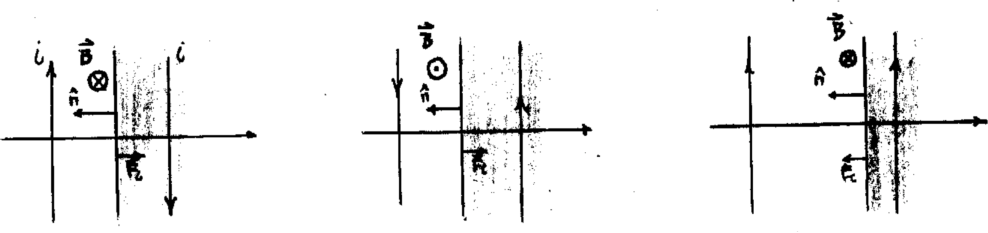
\includegraphics[width=0.9\textwidth]{images/fig_ft1_tensorM5.pdf}	 
	\end{center}
	\caption{}
\end{figure} 

Se llega al concepto de T cuando pensamos en campos para justificar las interacciones.
Para medios materiales se tendrán consecuentemente los siguientes tensores eléctrico
y magnético, respectivamente,
\[
	T_{ik} = \frac{1}{4\pi} \left[ E_iD_k - \frac{1}{2}\delta_{ik} \pe{D}{E}(1-b_e) \right] 
\]
\[
	T_{ik} = \frac{1}{4\pi} \left[ H_iB_k - \frac{1}{2}\delta_{ik} \pe{H}{B}(1-b_m)  \right] 
\]

Cuando T está diagonalizado la traza no es nula. Cuando se diagonaliza, ahciendo
\[
	| T - \lambda \mathbb{1} | = 0
\]
se tienen $\lambda_1 = E^2 / 8\pi$ y $\lambda_{2,3} = - E^2 / 8\pi$, donde el
autovector de $\lambda_1$ corresponde a la dirección de \vb{E} y $\lambda_{2,3}$
a las direcciones perpendiculares.
\[
	d\vb{F}|_{\parallel} = T\cdot d\vb{S}|_{\parallel} \rightarrow \frac{E^2}{8\pi} dS|_{\parallel}
\]
el campo eléctrico transmite una tensión $E^2/8\pi$ paralela a la dirección del campo.
El tensor diagonalizado es 
\[
	T = \frac{1}{4\pi}\begin{pmatrix}
	        E^2/2	& 0 	& 0 \\
		0	& -E^2/2	& 0 \\
		0	& 0	& -E^2/2
	       \end{pmatrix}
\]

% =================================================================================================
\section{Método cuasiestacionario}
% =================================================================================================

Se aproximan campos y fuentes con frecuencias bajas, es decir cuando $\omega \approx 0$.
Observemos que se desarrollará la parte espacial pero la temporal quedará como está.
Se considera
\[
	\vb{E}(\vb{x},t) = \vec{\mathbb{E}} \euler^{i\omega/c \hat{n}\cdot\vb{x}} \euler^{-i\omega t}
\]
y se desarrollará la parte espacial en torno a $\omega=0$. Comencemos el show,
\[
	\vb{E}(\vb{x},t) = \vec{\mathbb{E}} + \omega\frac{i\hat{n}\cdot\vb{x}}{c} \vec{\mathbb{E}} +
			\omega^2 \frac{i^2(\hat{n}\cdot\vb{x})^2}{c^2} \vec{\mathbb{E}}
\]
y si le {\it pegamos} la parte temporal será
\[
	\vb{E}(\vb{x},t) = \underbrace{ \vec{\mathbb{E}} \euler^{-i\omega t} }_{\vb{E}^{(0)}} + 
	\underbrace{\omega\frac{i\hat{n}\cdot\vb{x}}{c} \vec{\mathbb{E}}\euler^{-i\omega t}}_{\vb{E}^{(1)}} +
	\underbrace{\omega^2\frac{i^2(\hat{n}\cdot\vb{x})^2}{c^2}\vec{\mathbb{E}}\euler^{-i\omega t}}_{\vb{E}^{(2)}}
\]

Para el campo \vb{B} puede hacerse una descomposición análoga,
\[
	\rotorm{}(\vb{E}^0 + \vb{E}^1 + \vb{E}^2) = -\frac{1}{c} \dpar{}{t}(\vb{B}^0 + \vb{B}^1 + \vb{B}^2)
\]
\[
	0 + \underbrace{\rotorm{E}^1}_{\propto \omega } + \underbrace{\rotorm{E}^2}_{\propto \omega^2 } = 
	\underbrace{\frac{i\omega}{c}\vb{B}^0}_{\propto \omega } + \underbrace{\frac{i\omega}{c}
	\vb{B}^1}_{\propto \omega^2 } + \underbrace{\frac{i\omega}{c}\vb{B}^2}_{\propto \omega^3 }
\]
\[
	-\frac{1}{c}\dpar{\vb{B}}{t} = -\frac{1}{c}(-i\omega)\vec{\mathbb{B}}\euler^{-i\omega t}
	-\frac{1}{c}\omega(-i\omega)\frac{i\hat{n}\cdot\vb{x}}{c}\vec{\mathbb{B}}\euler^{-i\omega t}
	-\frac{1}{c}\frac{\omega^2}{2}(-i\omega)\frac{i^2(\hat{n}\cdot\vb{x})^2}{c^2}\vec{\mathbb{B}}\euler^{-i\omega t}
\]
\[
	-\frac{1}{c}\dpar{\vb{B}}{t} = \frac{i\omega}{c}\vb{B}^{(0)} 
	+ \frac{i\omega}{c} \underbrace{\frac{i\omega}{c}\vec{\mathbb{B}}\euler^{-i\omega t}}_{\vb{B}^{(1)}}
	+ \frac{i\omega}{c} \underbrace{ \left.\frac{\omega^2}{2}\frac{i^2(\hat{n}\cdot\vb{x})^2}	
	{c^2}\vec{\mathbb{B}} \euler^{-i\omega t}\right.}_{\vb{B}^{(2)}}
\]
Esto establece una equivalencia entre órdenes,
\[
	\rotorm{E}^{(0)} = 0 \qquad \qquad \rotorm{E}^{(1)} = -\frac{1}{c}\dpar{\vb{B}^{(0)}}{t}
\]
donde el orden cero es el de los campos estáticos.

\begin{sidewaystable}
	%\centering A table
	\begin{center}
	\begin{tabular}{|c|c|c|}
	\hline
	Orden cero & Orden uno & Orden dos \\
	\hline
	& & \\
	$\displaystyle{ \divem{}\epsilon\vb{E}^0 = 4\pi\rho^0 }$ & $ \divem{}\epsilon\vb{E}^{(1)} = 4\pi\rho^{(1)} $ 
	& $ \divem{}\epsilon\vb{E}^{(2)} = 4\pi\rho^{(2)} $  \\
	& & \\
	$ \rotorm{}\vb{E}^{(0)} = 0 $ & $\displaystyle{\rotorm{}\vb{E}^{(1)} = -\frac{1}{c} \dpar{\vb{B}^{(1)}}{t} }$ 
	& $ \displaystyle{ \rotorm{}\vb{E}^0 = -\frac{1}{c} \dpar{\vb{B}^{(2)}}{t} }$  \\
	& & \\
	$ \divem{}\vb{B}^{(0)} = 0 $ & $\divem{}\vb{B}^{(1)} = 0  $ & $ \divem{}\vb{B}^{(2)} = 0 $  \\
	& & \\
	$ \displaystyle{ \rotorm{}\frac{1}{\mu}\vb{B}^{(0)} = \frac{4\pi}{c}\vb{J}^{(0)} } $ 
	& $ \displaystyle{ \rotorm{}\frac{1}{\mu}\vb{B}^{(1)} = \frac{4\pi}{c}\vb{J}^{(1)} + 
	\frac{1}{c}\dpar{\epsilon\vb{E}^{(0)}}{t} } $ 
	& $ \displaystyle{ \rotorm{}\frac{1}{\mu}\vb{B}^{(2)} = \frac{4\pi}{c}\vb{J}^{(2)} +
	\frac{1}{c}\dpar{\epsilon\vb{E}^{(1)}}{t} } $  \\
	& & \\
	$ \divem{}\vb{J}^{(0)} = 0 $ & $\displaystyle{ \divem{}\vb{J}^{(1)} = -\dpar{\rho^{(0)}}{t} }$ 
	& $\displaystyle{ \divem{}\vb{J}^{(2)} = -\dpar{\rho^{(1)}}{t} } $  \\
	& & \\
	\hline
	\end{tabular} 
	\end{center}  
	%\caption{A caption}
\end{sidewaystable}

Consideramos $\omega/c \ell \ll 1$ con $\ell$ alguna longitud característica del sistema.
Esta es la aproximación del sistema para poder usar cuasiestacionario.

En general, en el método cuasiestacionario se alternarán para un mismo campo el valor constante
(no necesariamente cero) y alguna función de $(\vb{x}, t)$. Es decir, que si $E_par = cte.$
entonces $E_impar \neq cte.$ y si $B_impar \neq cte.$ entonces $B_par = cte.$

Recordemos que la nomenclatura de corrientes en 
\[
	\rotorm{H} = \frac{4\pi}{c}\vb{J} + \frac{1}{c}\dpar{\vb{D}}{t}
\]
es corriente de conducción y de desplazamiento respectivamente.

Cuando un conductor no es perfecto vale la ley de Ohm,
\[
	\vb{J} = \sigma \vb{E} \qquad  \delta = \frac{c^2}{2\pi\omega\sigma}
\]
donde $\delta$ es la profundidad pelicular, una longitud de penetración.



% \bibliographystyle{CBFT-apa-good}	% (uses file "apa-good.bst")
% \bibliography{CBFT.Referencias} % La base de datos bibliográfica

\end{document}
